\chapter[Remote Observations: Early-stages and Later-stages of Eruption]{Remote Observations\\\LARGE Early-stages and Later-stages of Eruption}
\label{chapter2}
This chapter focuses on the kinematics of CBFs in both the lower and middle/outer coronas, along with an examination of coronal plasma conditions during these eruptions. The chapter will present the results followed by a discussion and concluding remarks.

\section{Introduction}
CMEs are prominent indicators of solar activity, observable through various wavelengths including white light, UV, and radio \citep{vourlidas_2003, zhang_2006, bein_2011, bastian_2001, veronig_2010}. Early CME phases are effectively observed in Extreme Ultraviolet (EUV) light, facilitated by instruments like AIA aboard SDO \citep{lemen_2011, pesnell_2012}. CMEs can induce shock waves in the solar corona, visible as EUV waves or CBFs \citep{thompson_1998, long_2011}.

CBFs are disturbances propagating over the solar disk and limb, often faster than local characteristic speeds, driven primarily by CMEs or solar flares \citep{thompson_1998, veronig_2010, vrsnak_2008, magdaleni_2010, nindos_2011}. They appear as dome-shaped structures in radio and white-light observations, composed of denser plasma and thus appearing brighter in images \citep{pick_2006, nindos_2008, thompson_2009}.

Studies have clarified CBF characteristics both on the solar disk and off the limb, confirming their wave-like nature \citep{nitta_2013, long_2011, olmedo_2012}. Observations from instruments like LASCO onboard SOHO have extended shock wave investigations beyond 2.5 \rsun \citep{domingo_1995, vourlidas_2003}. While EUV observations link CMEs and EUV waves, understanding shock waves in EUV remains incomplete \citep{patsourakos_2009, kozarev_2011}. Emission measure modeling using AIA's EUV channels provides insights into temperature and density changes in the wavefront's sheath \citep{kozarev_2011}. Multi-wavelength observations from SOHO/LASCO and SDO/AIA instruments have revealed valuable information about CBF properties near the Sun \citep{warmuth_2015}.
Factors such as nearby active regions or coronal holes can distort CBF morphology, and a connection between CBFs and chromospheric disturbances known as Moreton waves has been established \citep{ofman_2002, mann_2003, piantschitsch_2018, thompson_1999b}.
In this study, I analyzed 26 CBF events up to \almost17\rsun using observations and modeling tools from the Solar Particle Radiation Environment Analysis and Forecasting--Acceleration and Scattering Transport (SPREAdFAST) framework \citep{kozarev_2022}. The study aims to characterize CBF kinematics and estimate ambient plasma properties to understand the relationships between shock and plasma parameters.

\section{EUV Observations}
We conducted a study utilizing data from the SOHO/ERNE instrument, focusing on proton events with energies between 17-22 MeV, spanning from 2010 to 2017. Initially, 216 events were identified, but after stringent selection criteria were applied, 133 events were excluded due to various factors such as the absence of EUV wave associations, CMEs, or flares. This left us with a final set of 26 events for analysis.
The selected events, previously discussed in \citep{kozarev_2022}, were further examined using imagery from the AIA instrument's EUV channel 193 $\AA$. These images, captured at a 24-second cadence, provided the primary input for our analysis within the SPREAdFAST framework.

Detailed information about the selected events, including their start/end times, associated flares, and source locations on the solar disk, was obtained from the Heliophysics Events Knowledge (HEK) database. Notably, the mean latitude and longitude of the CBFs were calculated, along with their distribution across the solar hemispheres and quadrants.
CBFs, observed as faint quasi-spherical sheaths, were primarily visible in the 193 $\AA$ channel. To analyze their evolution, sequences of base-difference images were generated for each event, allowing us to track their propagation over time \citep{vourlidas_2003, ontiveros_2009, kozarev_2011, ma_2011}.
The mean latitude and mean longitude of the CBFs were calculated as 56.35 and 378.04 arcsec, respectively. Additionally, the mean latitudes of CBFs in the northern and southern solar hemispheres were found to be 283.00 and -252.73 arcsec, respectively. As for the mean longitudes, they were -775.71 and 803.11 arcsec on the eastern and western sides, respectively.

To analyze the kinematics of CBFs, the Coronal Analysis of SHocks and Waves framework \citep[CASHeW]{kozarev_2017} was employed. This semi-automated technique involved extracting annular regions from AIA images and mapping them onto polar projections (Fig.~\ref{fig_annplot}). By tracking intensity changes along radial and lateral directions, we could measure the kinematics of the CBFs.

Furthermore, plasma parameters and modeling were performed using information retrieved from the HEK database and Nariaki Nitta's catalog of coronal waves \citep{nitta_2013}. The SPREAdFAST framework facilitated calculations of kinematics, inference of shock parameters, and determination of plasma properties for each event.

\begin{figure}[!htp] % updated!
	\centerline{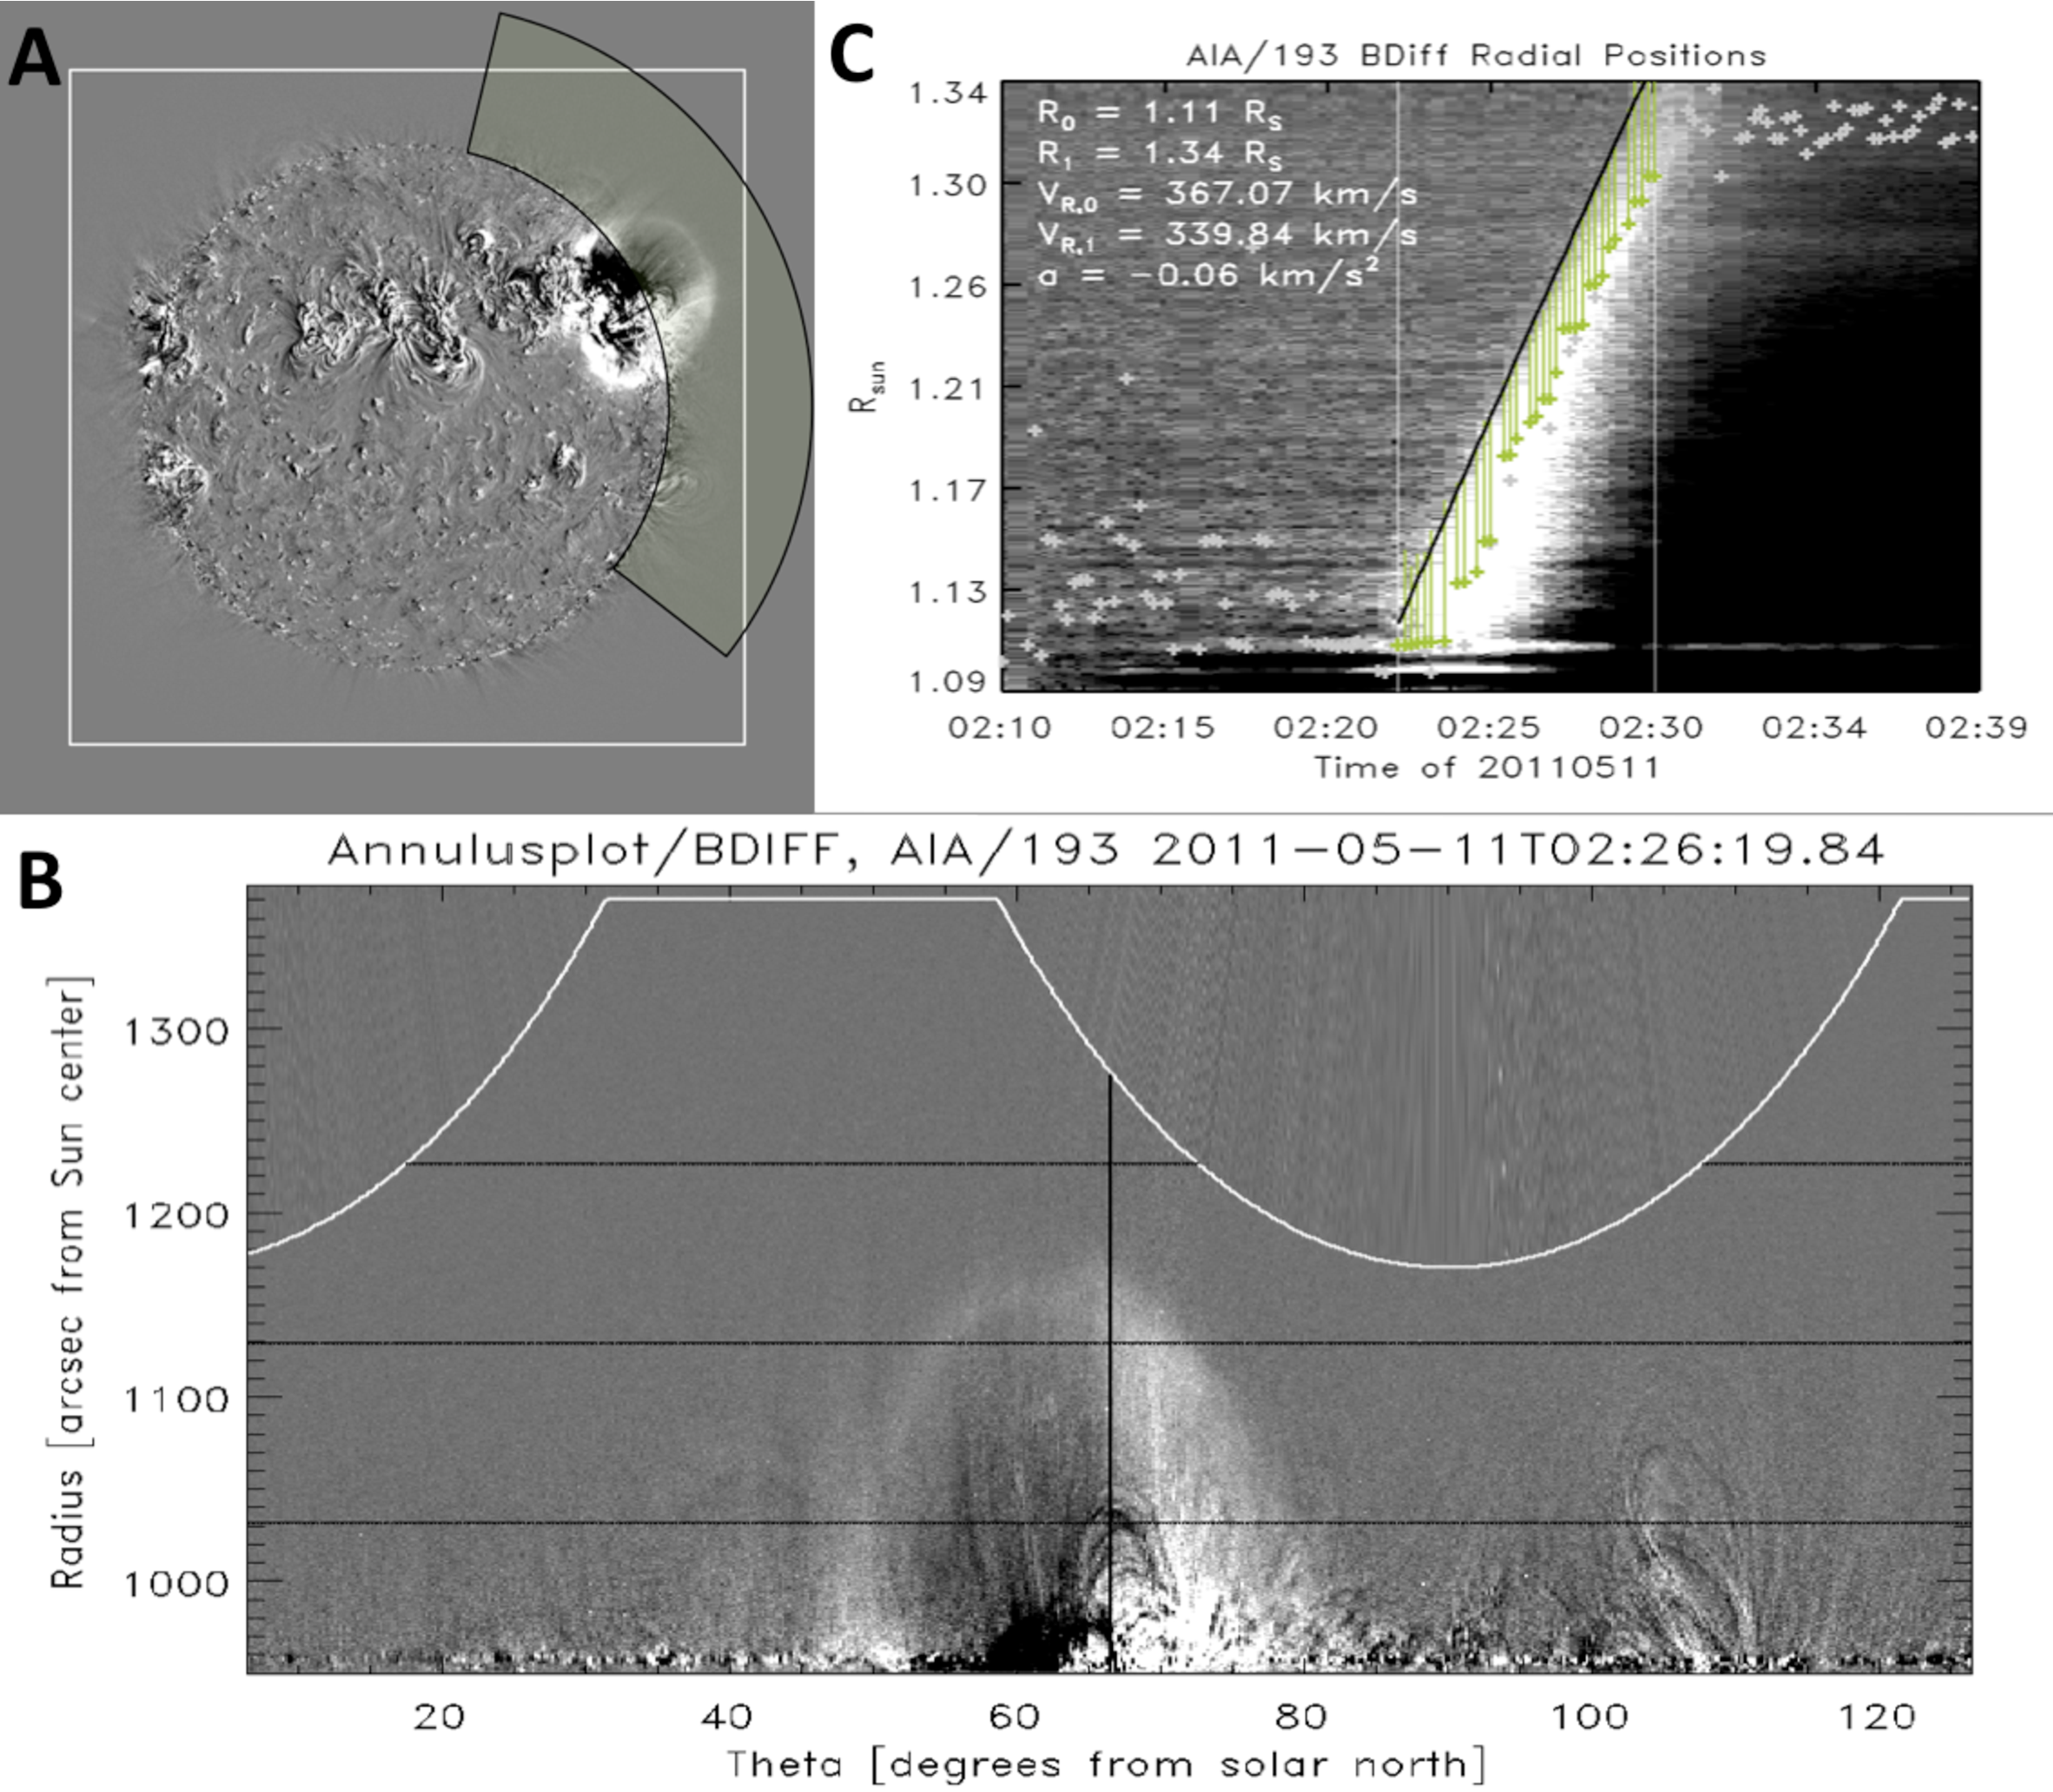
\includegraphics[width=0.9\columnwidth]{chapter2/figs/fig_annplot.pdf}}
	\caption{Illustration for the annulus method used to extract kinematic data from AIA images. (A) shows the full Sun disk with the relevant region highlighted for analysis (green sector). The white box outlines the AIA FOV. (B) displays the extracted annular region mapped onto polar coordinates, with the actual data extent marked by the white curve. Black lines indicate the directions used for measuring radial and lateral motions. (C) shows a stacked plot of intensity along the radial direction, with green markers highlighting intensity peaks and their corresponding distances from the CBF wavefront. The white lines represent the time interval during which the CBF is tracked within the AIA FOV. This figure is curated from \citep{kozarev_2017}.}
	\label{fig_annplot}
\end{figure}

To accurately determine the positions of CBFs over time, we employed several algorithms, including Savitzky-Golay filtering \citep{savitzky_1964} for data smoothening and local minima/maxima ordering for identifying wave positions. Additionally, we manually specified starting and ending times for each CBF event and determined their corresponding heights above the solar limb.
By analyzing intensity values, we defined the positions of CBFs at each time step, considering the front and back of the wave to be at 20\% of the peak intensity. Furthermore, we applied mathematical techniques such as Levenberg-Marquardt least squares minimization \citep{markwardt_2009} and bootstrapping optimization \citep{efron_1979} to fit fourth-order polynomials to the wave positions, enabling measurements of speeds, accelerations, intensities, and thicknesses in both radial and lateral directions.

Finally, measurements of CBF heights and lateral positions were obtained relative to the solar disk and wavefront direction, respectively, providing comprehensive insights into the dynamics of these solar phenomena.
For further reference, the HEK database\footnote{HEK Database: \url{www.lmsal.com/isolsearch}}, Nariaki Nitta's catalog of coronal waves\footnote{Nariaki Nitta's Catalog: \url{https://lmsal.com/nitta/movies/AIA_Waves/index.html}}, and the LASCO CME Catalog\footnote{LASCO CME Catalog: \url{https://cdaw.gsfc.nasa.gov/CME_list/}} were utilized, along with detailed summary plots available in the online SPREAdFAST catalog\footnote{SPREAdFAST Catalog: \url{https://spreadfast.astro.bas.bg/catalog/}}.

\section{Data Analysis and Methods}
The Solar Particle Radiation Environment Analysis and Forecasting–-Acceleration and Scattering Transport (SPREAdFAST) system, developed by \citet{kozarev_2022} and referred to as SPREAdFAST throughout this discussion, operates as a physics-based prototype for forecasting SEP events within the heliosphere. Built upon the CASHeW framework, SPREAdFAST integrates data-driven models to forecast various aspects of SEP events, including arrival times, maximum intensities, and fluxes at different locations in the inner heliosphere. These predictions play a vital role in space weather forecasting, contributing to the protection of assets owned by the European Space Agency (ESA) and aiding satellite operators in making informed decisions to mitigate the impacts of space weather on electronics and human activities in space \citep{kozarev_2022}.

The SPREAdFAST catalog offers summary plots of J-maps and kinematic data for each SEP event, as highlighted by \citet{kozarev_2022}. Additionally, to ensure consistency in lateral kinematic measurements, an averaging technique is applied to data from both lateral left and right flanks, as described by the same authors. Further analysis involves the application of a Savitzky-Golay fit, as outlined in previous work by \citet{kozarev_2019}, and the utilization of analytical models for CME kinematics by \citet{gallagher_2003} and \citet{byrne_2013} to extrapolate smoothed radial positions up to $\sim$17\rsun.

Moving forward, the development of synthetic shock models (S2M) forms the next phase of the study, as mentioned by \citet{kozarev_2022}. These models, operating at a 24-second cadence, are constructed based on extrapolated radial and lateral kinematic results and incorporate major and minor axes of spheroids representing compressive waves. The shock surface is delineated from the onset of the CBF until its nose reaches 10 \rsun and then extended up to 30 \rsun utilizing results from the Magnetohydrodynamic Algorithm outside a Sphere (MAS) synoptic coronal model.

The methodology for estimating shock density jump is detailed by \citet{kozarev_2017}, involving the calculation of differential emission measure (DEM) during and before the event at each shock crossing and timestep. This approach, informed by \citet{cheung_2015}, provides insights into the variation in density across shock structures. Notably, while the density jump within the AIA FOV typically remains below 1.2, regions beyond observational limits are assigned a value of 1.2, assuming the presence of weak shocks.
To facilitate analysis, the synthetic shock model is segmented into distinct regions--the cap representing the shock nose, Zone 1, and Zone 2 representing the shock flanks--as explained by \citet{kozarev_2022}. This segmentation aids in the examination of plasma parameter distributions across different sectors of the shock surface, as depicted in Figure~\ref{fig_segments}.

\begin{figure}[!htp] % updated!
	\centerline{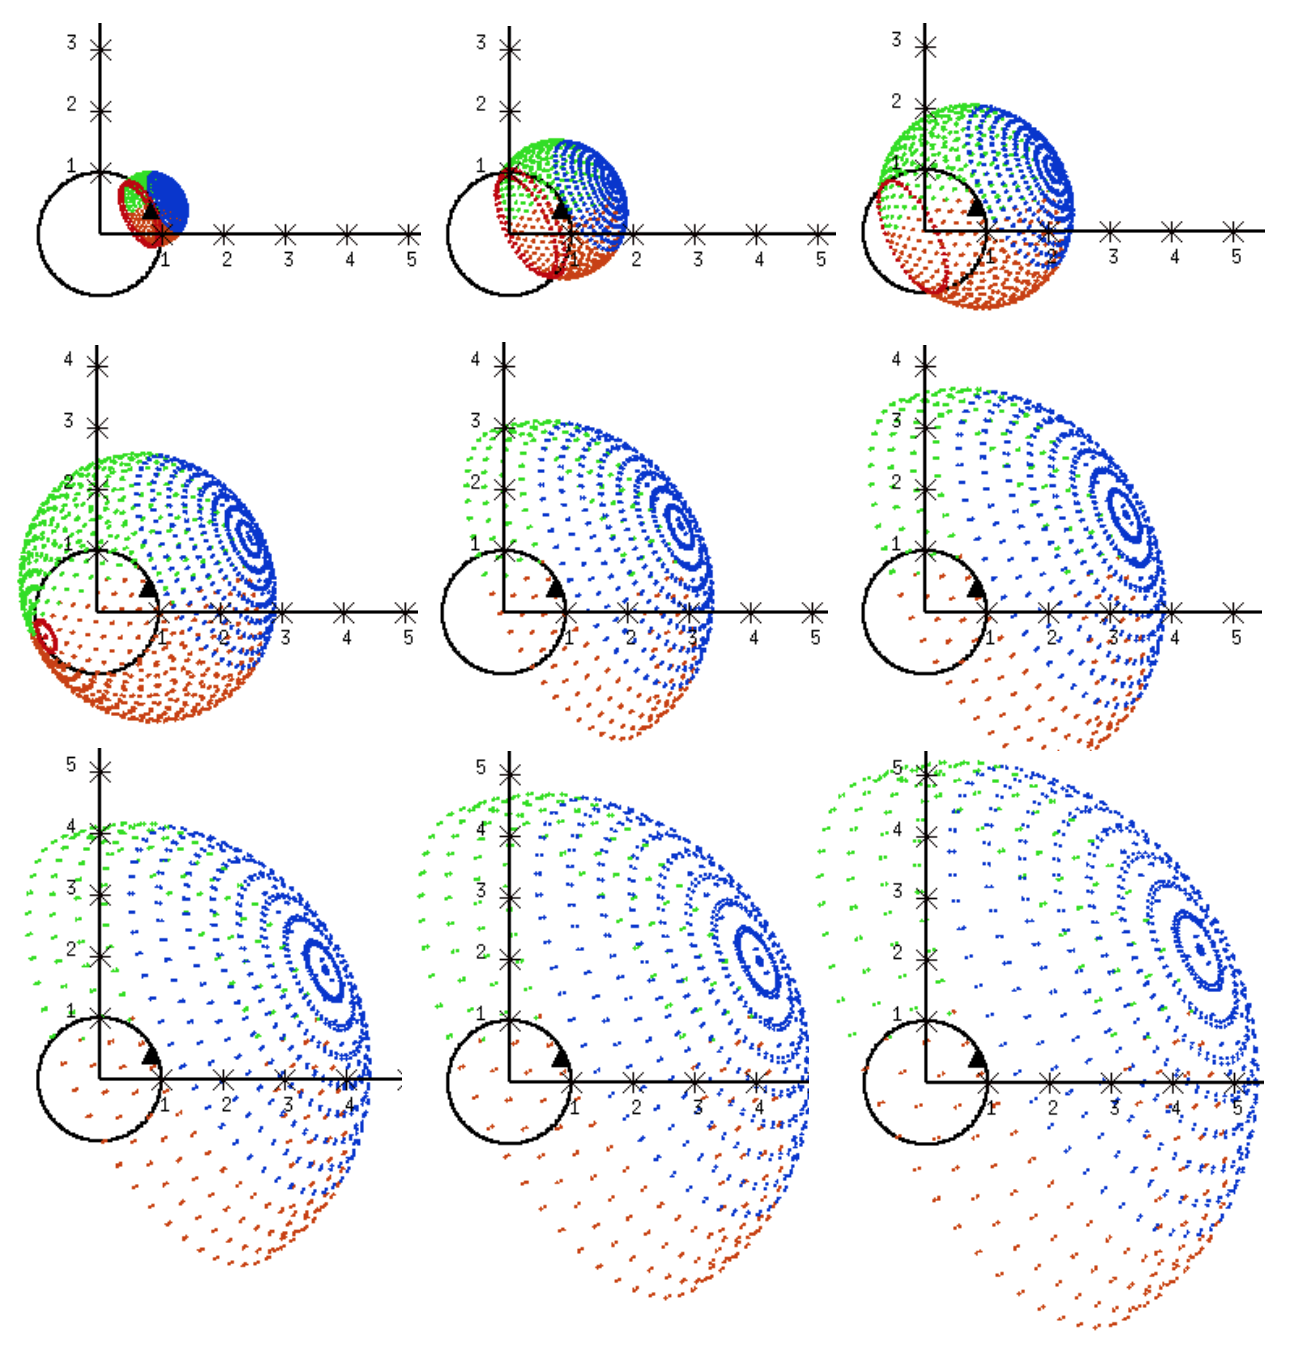
\includegraphics[width=0.5\columnwidth]{chapter2/figs/fig_s2m_segments_geometry.png}}
	\caption{Synthetic shock model divided into three segments; the cap zone in blue and the flank zones are in red and green.}
	\label{fig_segments}
\end{figure}

\section{CBF Kinematics and Geometric Modeling: Case Study May 11, 2011}
In this section, I analyze a case study event in the low corona region and investigate plasma parameters along shock-crossing magnetic field lines in the AIA FOV.

\subsection{Event Context}
The eruption occurred on May 11, 2011, at around 02:20 UT (Fig.~\ref{fig_aia_event}), originating from an active region in the northwestern sector (N18W52). It involved a massive shock wave propelled by a fast partial-halo CME, with a linear speed of 745 \kms, a 2$^{nd}$-order speed at 20\rsun of 776 \kms, and an acceleration of 3.3 m s$^{-2}$. The eruption was accompanied by a weak B8.1 solar flare and an eruptive filament observed by the SDO/AIA instrument.
Additionally, a type II radio burst was associated with the eruption, observed by the Learmonth spectrogram. Proton fluxes near 1 AU showed an increase, and an SEP event was detected at Earth with onset time of 03:39 UT and a $J_p$ of 0.0133 protons/(cm$^2$ s sr MeV) in the energy channel 17-22 MeV \citep{miteva_2016, miteva_2017}.  $J_p$ is the peak proton intensity after subtracting the pre-event level.

\begin{figure}[!htp] % updated!
	\centerline{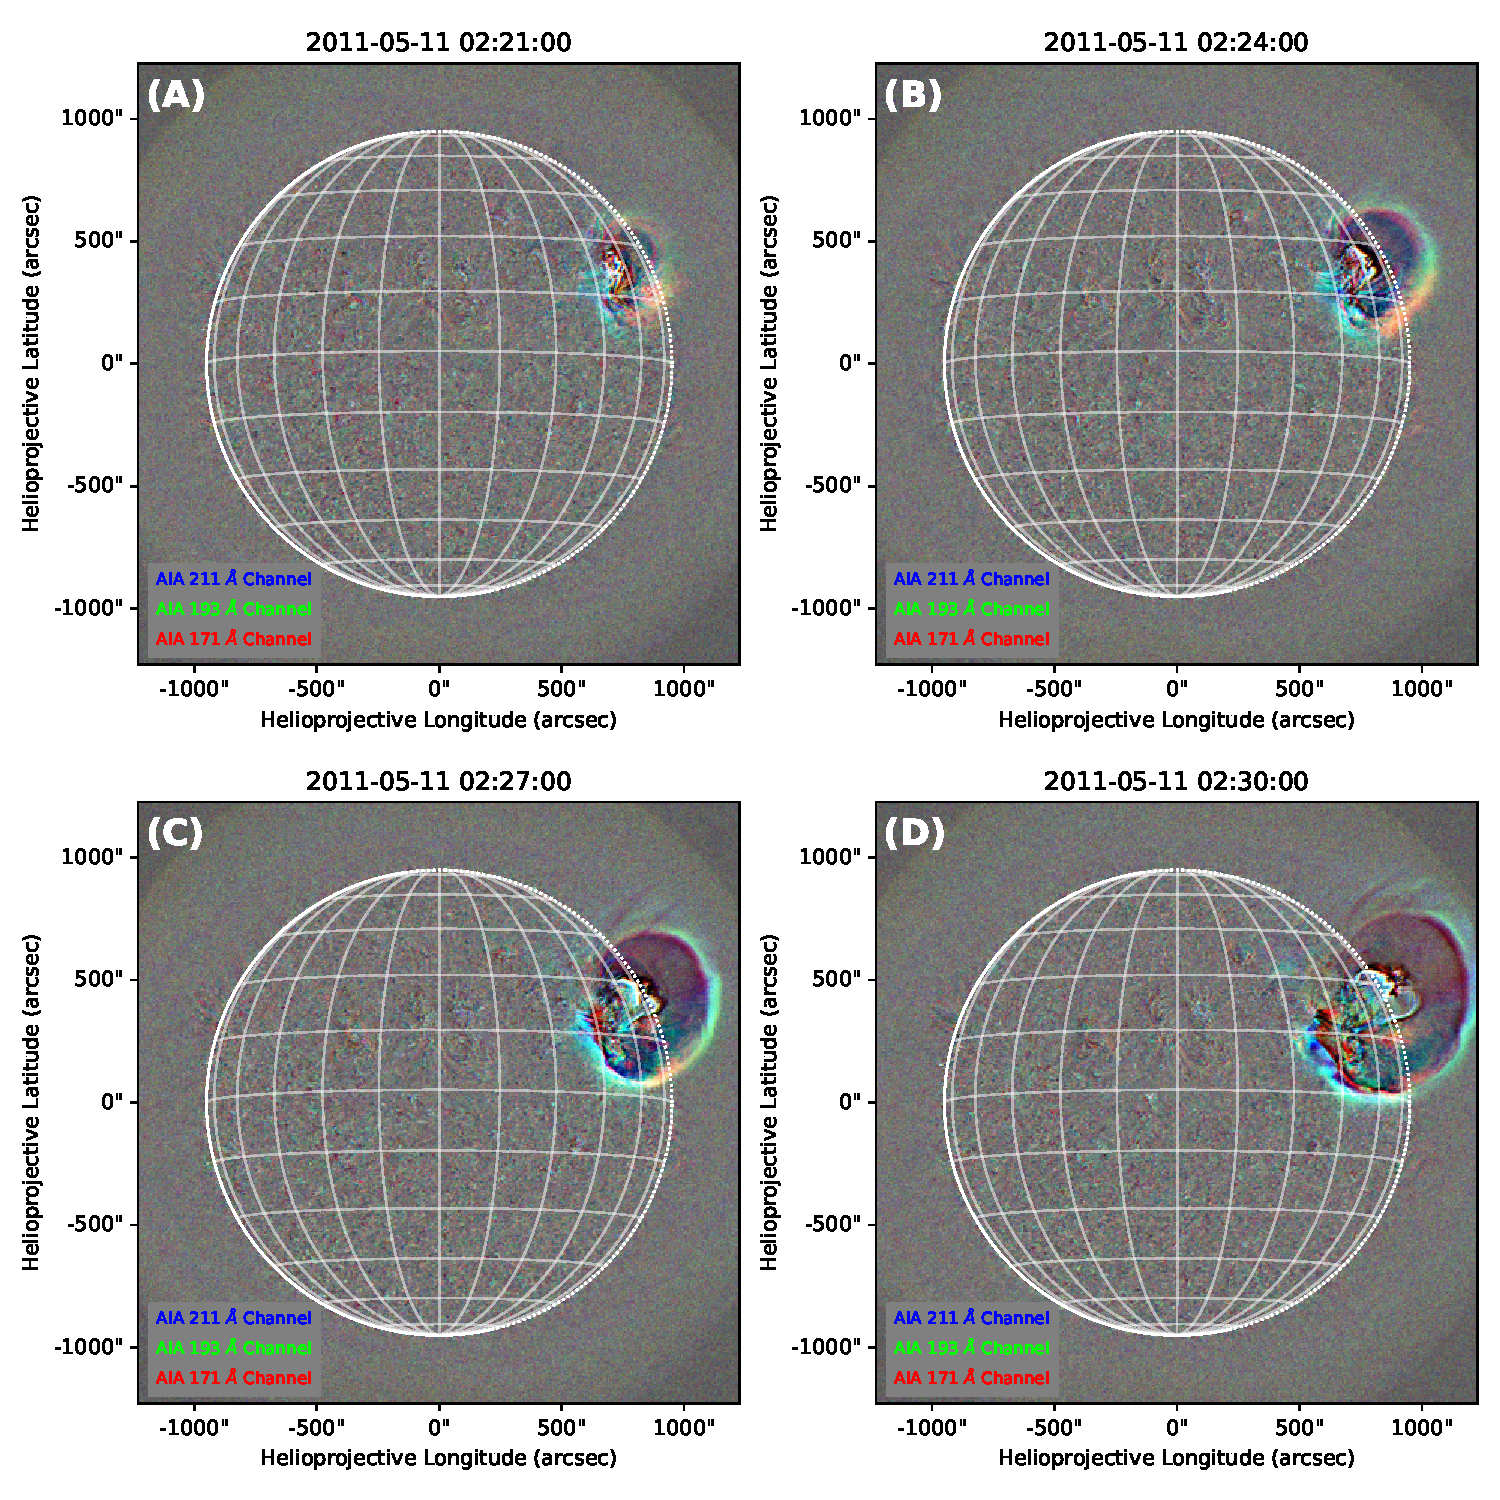
\includegraphics[width=0.8\columnwidth]{chapter2/figs/RGB_panel.pdf}}
	\caption{AIA running-difference images capture a coronal wave evolving over 9 minutes near the Sun's western limb, exhibiting markedly changing intensity and structure as observed in 171, 193, and 211 $\AA$.}
	\label{fig_aia_event}
\end{figure}

\subsection{Low Corona Part}
To investigate the kinematics of the CBF event, I employed the CASHeW module within the SPREAdFAST framework. The shock wave's asymmetrical evolution is detailed, along with its morphological changes over time. The average speeds and accelerations for the radial and lateral directions are provided (Fig.~\ref{fig_kinematics_110511}), along with a comparison of wave thickness between flanks. The shock surface is divided into segments for further analysis (Fig.~\ref{fig_segments}). Table~\ref{T_110511} provides a summary of the statistical results, and the results for the three segments are summarized in Table~\ref{T_sh_param_110511}.
Moreover, shock-crossing magnetic field lines during this event were investigated in \citep{kozarev_2022}, with key plasma parameters analyzed up to 10\rsun. The aspect ratio of the coronal wave's geometry is discussed, along with changes in shock-field angle and magnetic field amplitude over time and radial distance.

\begin{figure}[!htp] % updated!
	\centerline{
		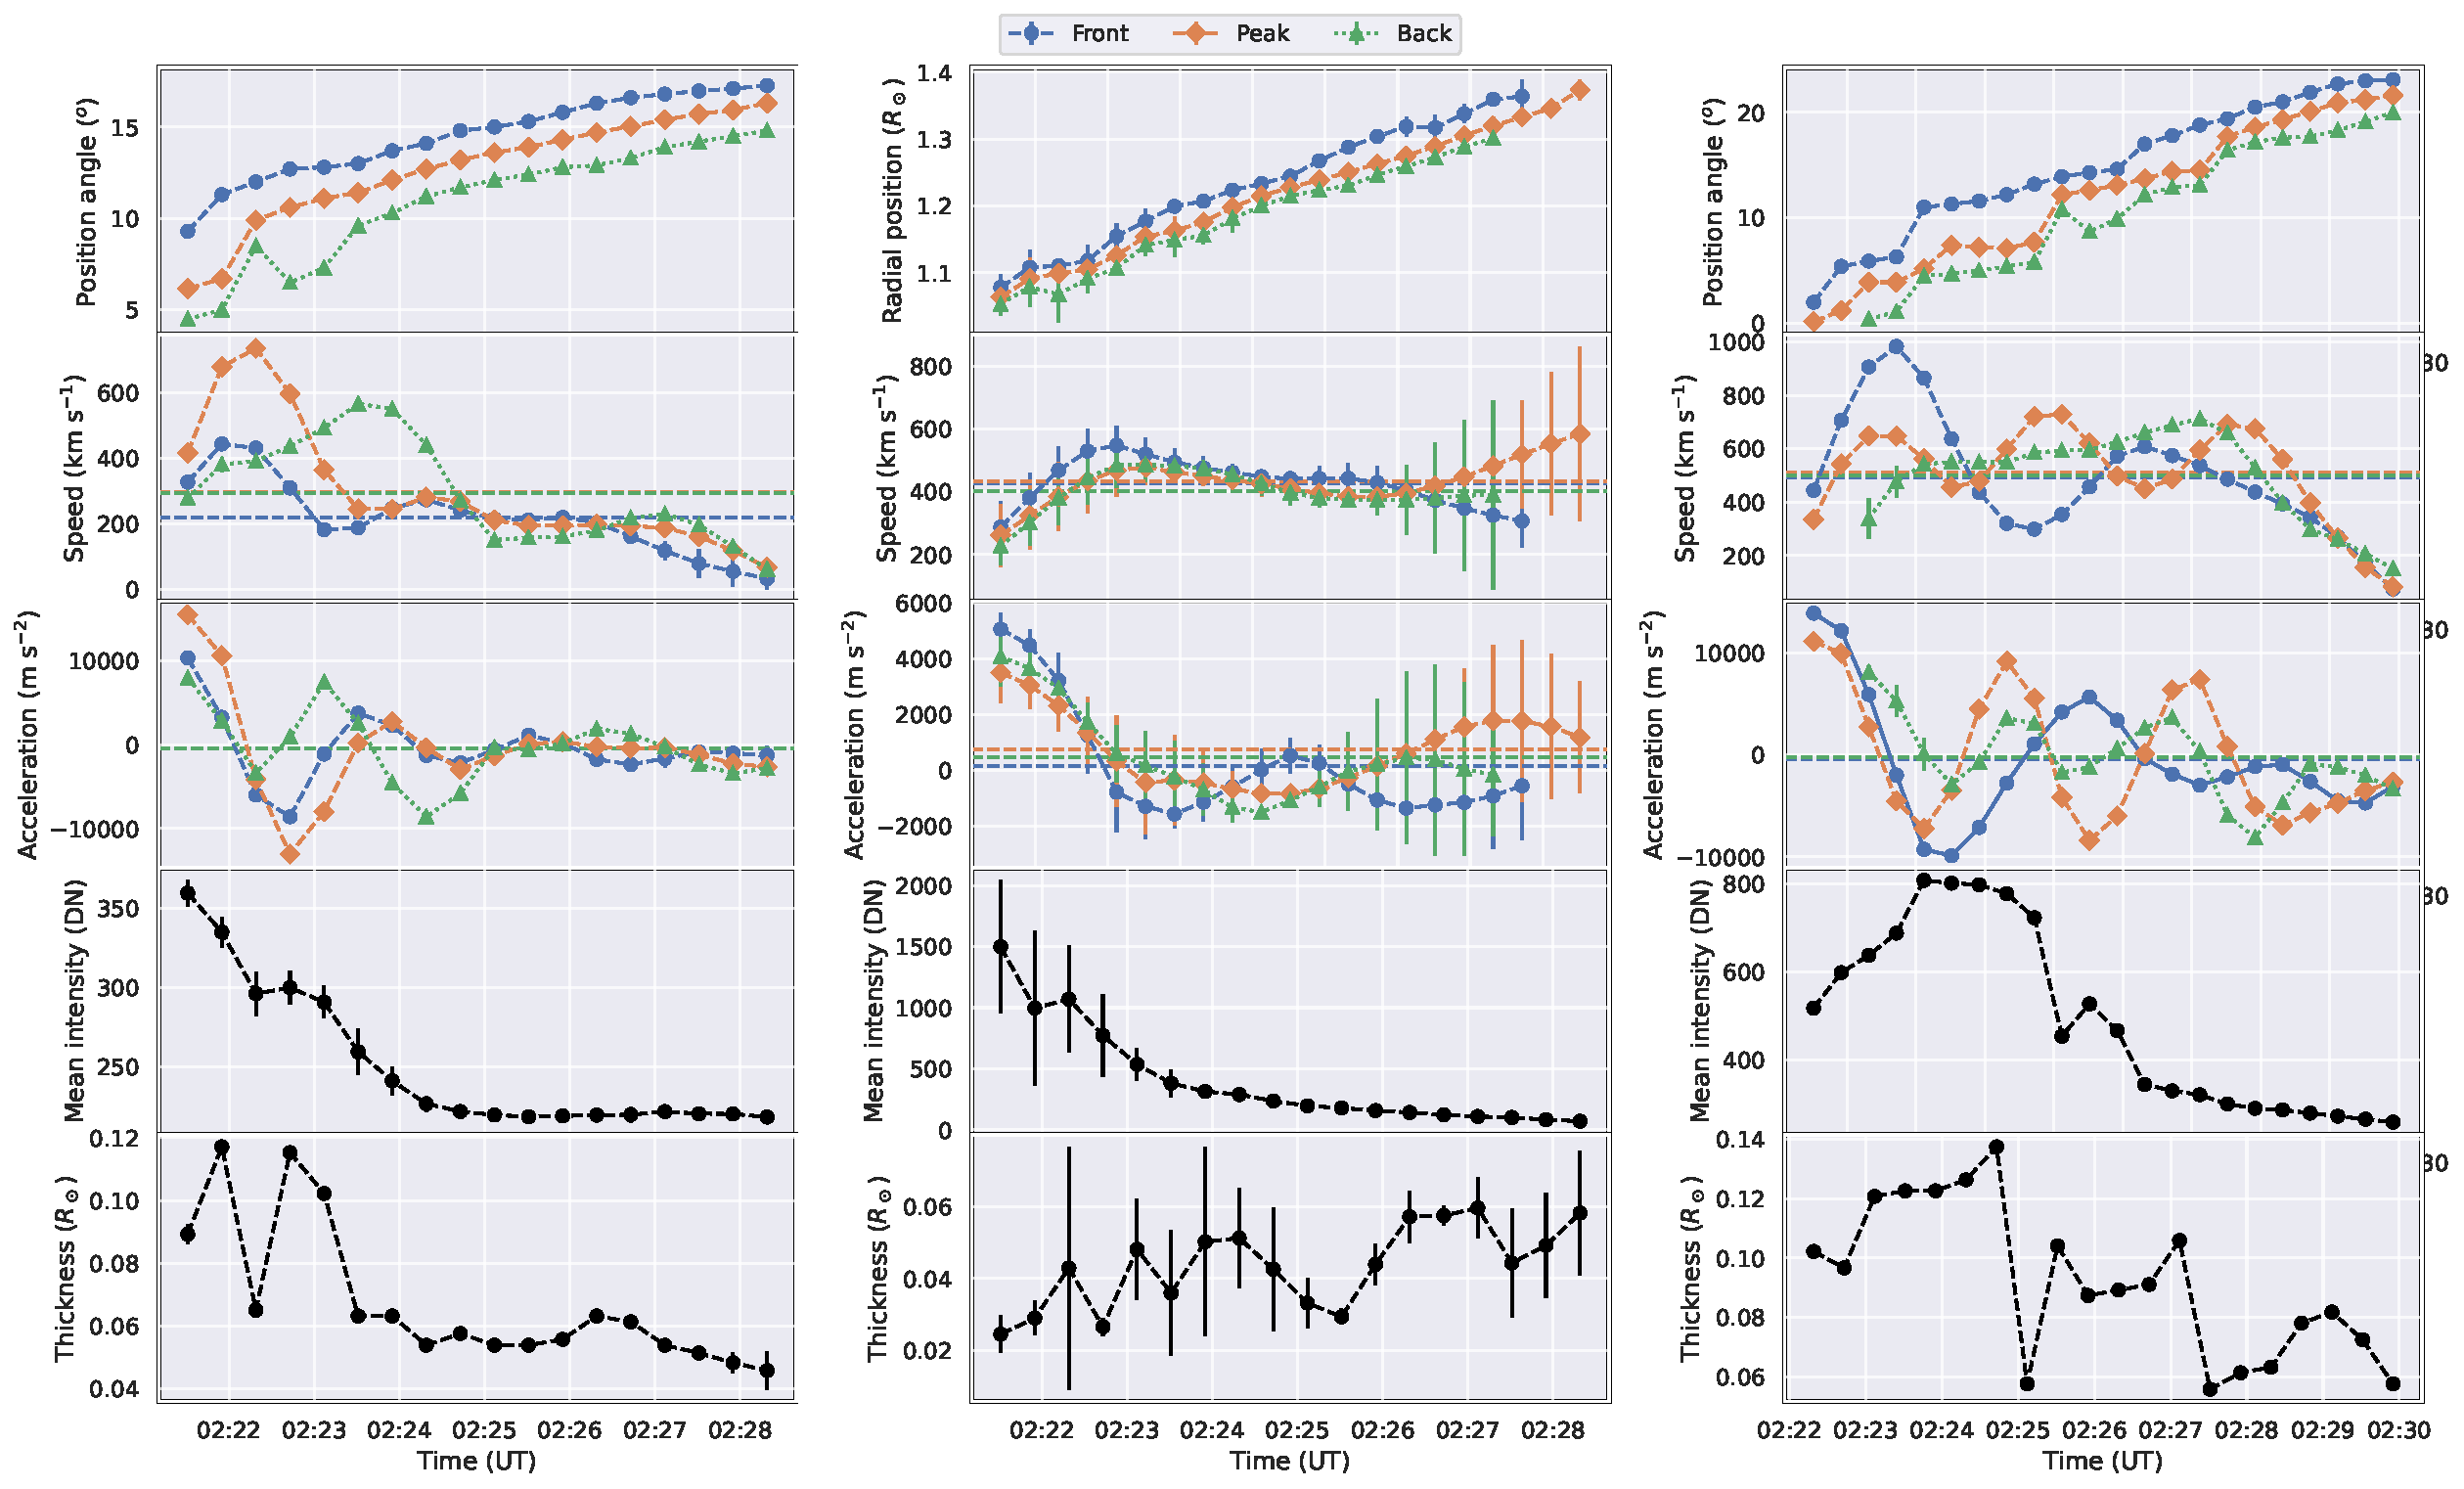
\includegraphics[width=1\textwidth,clip=]{chapter2/figs/euvwave_kinematics_110511_01.pdf}
	}
	\caption{Time-series kinematics of the CBF parameters for the front, peak, and back positions in the AIA FOV, with measurement uncertainties shown as small bars over the data points. The horizontal lines in the speed and acceleration panels denote the mean speeds and accelerations for the wave front, peak, and back with respective colors. The left and right columns represent the lateral kinematic measurements in the left and right flanks of the wave, respectively. The middle column represent the kinematic measurements in the radial direction.}
	\label{fig_kinematics_110511}
\end{figure}

\begin{table}[!htp] % updated!
	\centering
	\caption{Mean values and their standard deviation of the wave parameters in the radial direction and the lateral direction for the left and right flanks, at the front, peak, and back sides of the wave for the event occurred on May 11, 2011, in the SDO/AIA FOV.}
	\label{T_110511}
	\resizebox{\textwidth}{!}{%
		\begin{tabular}{lc|c|c|c}
			\hline
			Parameter                              & Direction  & Front              & Peak                   & Back                 \\ \hline
			\multirow{3}{*}{$<speed>$ \kms}        & Lat. Left  & 218.46 $\pm$ 9.04  & 297.46 $\pm$ 5.45      & 293.94 $\pm$ 9.04    \\ \cline{2-5}
			& Radial     & 427.46 $\pm$ 51.85 & 433.11 $\pm$ 82.86     & 400.81 $\pm$ 83.78   \\ \cline{2-5} 
			& Lat. Right & 494.69 $\pm$ 0.00  & 509.25 $\pm$ 1.02      & 498.97 $\pm$ 9.21    \\ \hline
			\multirow{3}{*}{$<accel.>$ m s$^{-2}$} & Lat. Left  & -414.62 $\pm$ 227.23 & -401.46 $\pm$ 164.62 & -385.77 $\pm$ 227.23 \\ \cline{2-5}
			& Radial     & 147.41 $\pm$ 1009.19 & 758.97 $\pm$ 1287.65 & 485.38 $\pm$ 1365.80 \\ \cline{2-5} 
			& Lat. Right & -415.04 $\pm$ 0.00   & -209.81 $\pm$ 22.32  & -266.68 $\pm$ 250.80 \\ \hline
			\multirow{3}{*}{$<intensity>$ DN}      & Lat. Left  & \multicolumn{3}{c}{250.60 $\pm$ 5.90}               \\ \cline{2-5}
			& Radial     & \multicolumn{3}{c}{403.34 $\pm$ 143.30}             \\ \cline{2-5}
			& Lat. Right & \multicolumn{3}{c}{489.04 $\pm$ 2.86}               \\ \hline
			\multirow{3}{*}{$<thickness>$\rsun}   & Lat. Left  & \multicolumn{3}{c}{0.07 $\pm$ 0.00}                 \\ \cline{2-5}
			& Radial     & \multicolumn{3}{c}{0.04 $\pm$ 0.01}                 \\ \cline{2-5}
			& Lat. Right & \multicolumn{3}{c}{0.09 $\pm$ 0.00}                 \\ \hline
		\end{tabular}%
	}
\end{table}

\begin{table}[!htp] % updated!
	\centering
	\caption{Mean, median, and standard deviation of the shock parameters output, from the interaction of the S2M spheroid with the MAS MHD model results, for the shock's cap and flanks and for the whole shock surface, for the event on May 11, 2011.}
	\label{T_sh_param_110511}
	\begin{tabular}{lcccc}
		\hline
		\multirow{2}{*}{Segment} & \multirow{2}{*}{Parameter} & \multicolumn{3}{c}{Statistics} \\
		&                         & Mean & Median & Stdv \\ \hline
		All & $V_{SHOCK}$ \kms    & 577.77 & 578.39 & 72.79 \\ 
		& $\theta_{BN}$ \degree   & 70.06 & 0.63 & 44.83 \\ 
		& $B_{MAG}$ G             & 0.046 & 0.038 & 0.070 \\ 
		& Density Jump            & 1.193 & 1.188 & 0.185 \\ \hline
		
		Cap & $V_{SHOCK}$ \kms    & 555.18 & 550.86 & 42.46 \\ 
		& $\theta_{BN}$ \degree   & 19.37 & 3.61 & 25.51 \\ 
		& $B_{MAG}$ G             & 0.046 & 0.036 & 0.070 \\ 
		& Density Jump            & 1.193 & 1.188 & 0.015 \\ \hline
		
		Zone 1 & $V_{SHOCK}$ \kms & 613.69 & 609.32 & 59.42 \\ 
		& $\theta_{BN}$ \degree   & 6.46 & 0.21 & 50.92 \\ 
		& $B_{MAG}$ G             & 0.045 & 0.045 & 0.066 \\ 
		& Density Jump            & 1.190 & 1.187 & 0.008 \\ \hline
		
		Zone 2 & $V_{SHOCK}$ \kms & 631.37 & 614.23 & 73.07 \\ 
		& $\theta_{BN}$ \degree   & 0.10 & 0.51 & 10.61 \\ 
		& $B_{MAG}$ G             & 0.046 & 0.029 & 0.071 \\ 
		& Density Jump            & 1.194 & 1.188 & 0.016 \\ \hline
	\end{tabular}
\end{table}

\subsection{Middle/Outer Corona Part}
Complementary measurements from the SOHO/LASCO instrument\footnote{LASCO CME Catalog: \url{https://cdaw.gsfc.nasa.gov/CME_list/}} expand the analysis of EUV waves' kinematics in the middle/outer corona. The height-time profile of the CME leading edge associated with the coronal wave is examined, employing fitting models of \citet{gallagher_2003} and \citet{byrne_2013} to analyze the data (Fig.~\ref{fig_height_profile_aialasco_110511}). Insights into the wave's acceleration and speed variation over time and distance from the Sun are provided (Fig.~\ref{fig_rad_kinematics_aialasco_110511}).

\begin{figure}[!htp] % updated!
	\centerline{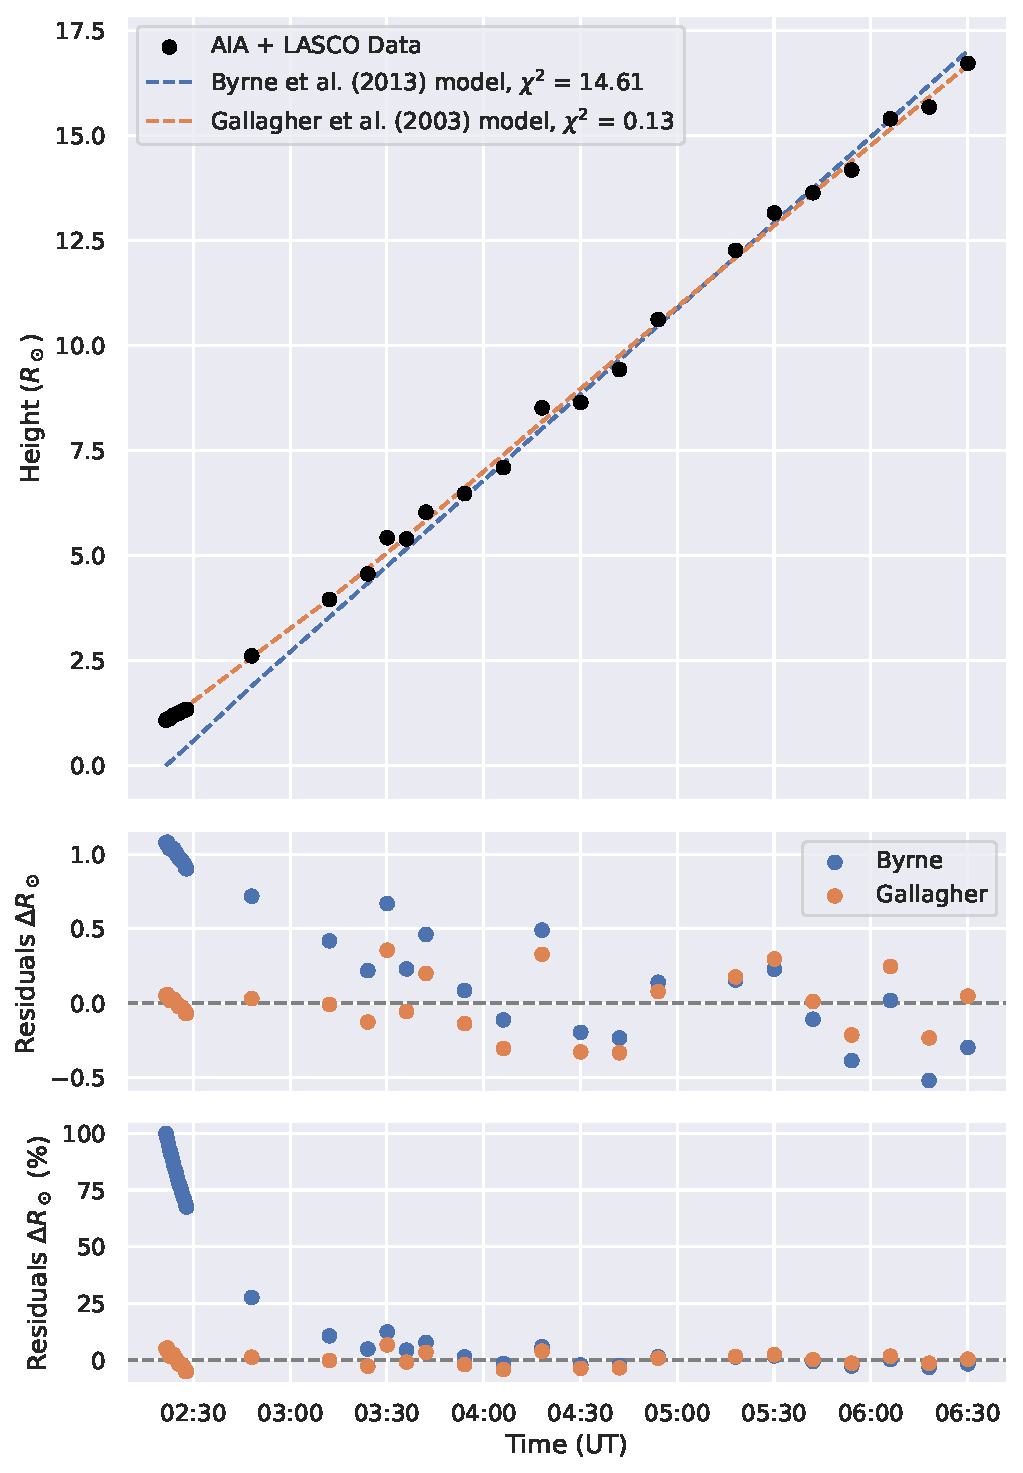
\includegraphics[width=0.6\columnwidth]{chapter2/figs/height_profile_residuals_aia_lasco_110511_01.pdf}}
	\caption{Top panel -- Height-time profile compiled from AIA and LASCO measurements for the event occurred on May 11, 2011, fitted with two CME kinematics models from the photosphere up to 17\rsun. Middle panel -- Difference between the fitting and the real observations. Bottom panel -- Relative residuals in \%.}
	\label{fig_height_profile_aialasco_110511}
\end{figure}

\begin{figure}[!htp] % updated!
	\centerline{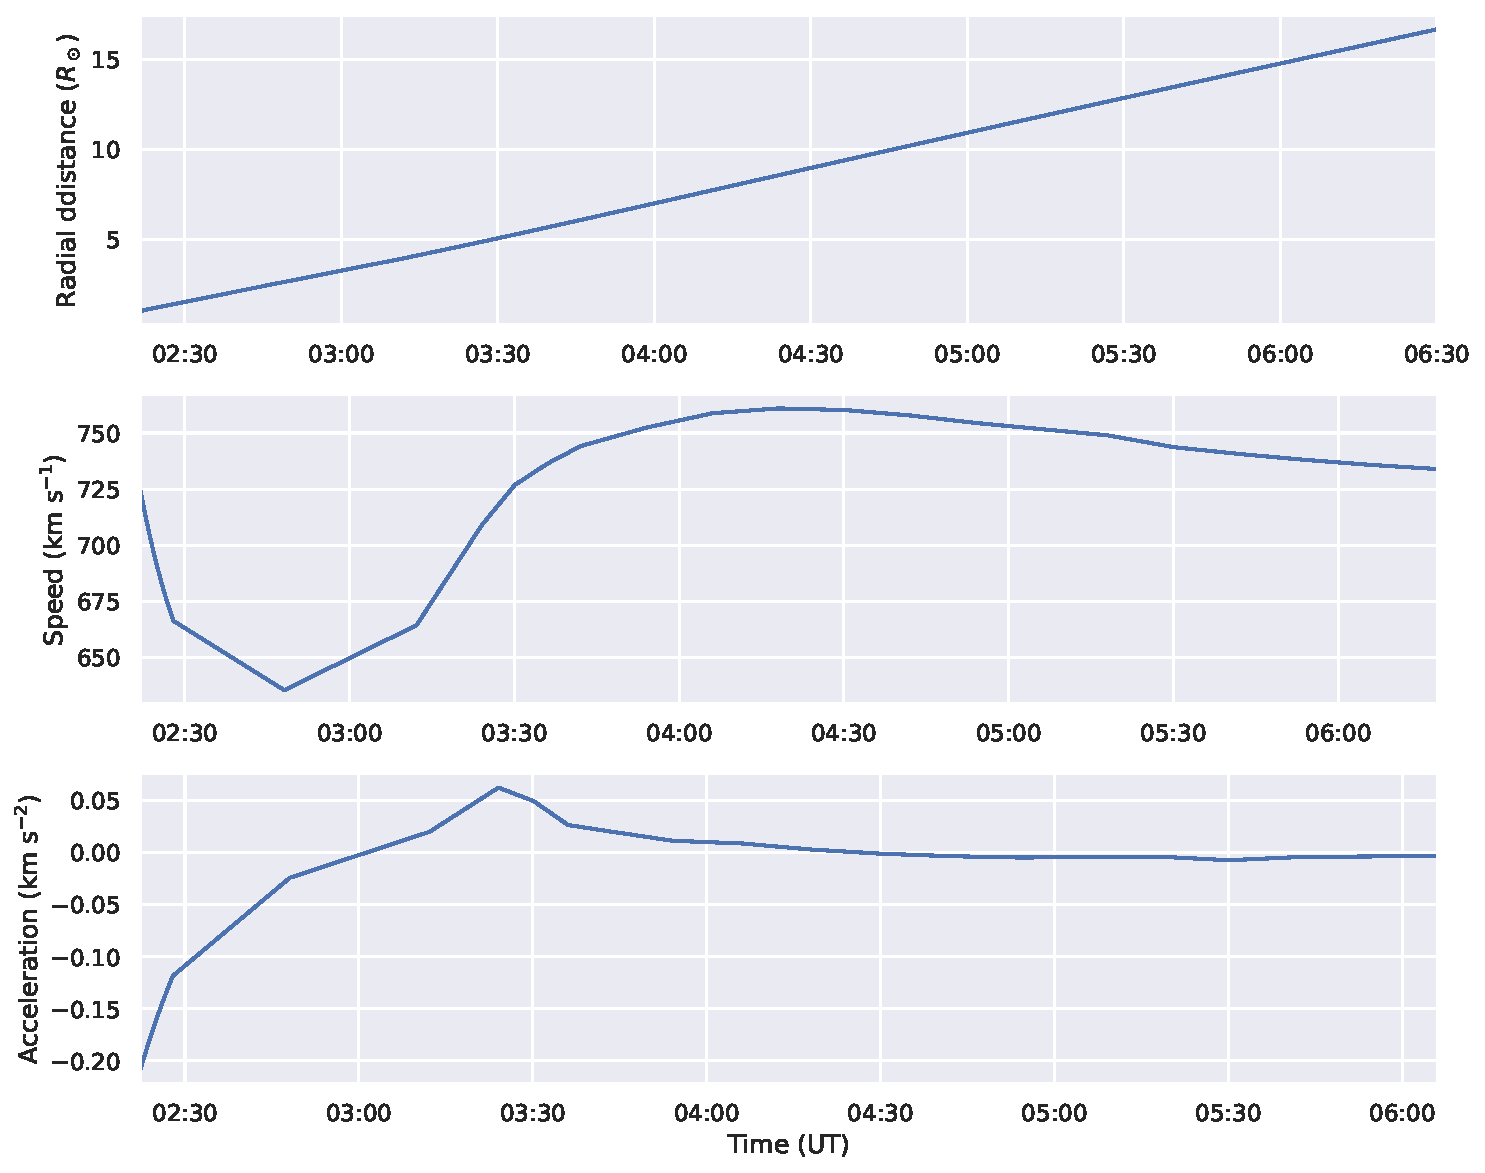
\includegraphics[width=0.8\columnwidth]{chapter2/figs/radial_kinematics_aia_lasco_110511_01.pdf}}
	\caption{Extrapolated radial kinematics for the event occurred on May 11, 2011, based on the ballistic model of \cite{gallagher_2003} up to 17\rsun.}
	\label{fig_rad_kinematics_aialasco_110511}
\end{figure}

\section{Statistical Study}
I conduct a thorough statistical analysis of coronal wave events observed in the AIA and LASCO FOVs, focusing on kinematic characteristics and plasma parameters.

Table~\ref{T_sh_param_all} summarizes statistical parameters related to shock characteristics, such as wave speed, intensity, and thickness in the AIA FOV.
Analysis reveals higher speeds, accelerations, lower mean intensities, and thickness in the radial direction compared to the lateral direction, suggesting early elongation of waves near the Sun.
Figure~\ref{fig_kinematics_spect_hist} illustrates EUV waves' kinematics evolution in the AIA FOV, showing parameter distributions as a function of distance for shock speed, acceleration, wave intensity, and thickness in radial and lateral directions.
Speed and intensity decline with distance due to momentum loss and decreasing plasma densities. All dynamic spectra for individual events are accessible on the SPREAdFAST catalog webpage\footnote{SPREAdFAST Catalog: \url{https://spreadfast.astro.bas.bg/catalog/}}.

\begin{table}[!htp] % updated!
	\centering
	\caption{Statistics of the EUV wave kinematics in the SDO/AIA FOV for the 26 events. LL and LR refer to the lateral left and right flanks, respectively. Rad refer to the radial front direction.}
	\label{T_sh_param_all}
	\resizebox{\textwidth}{!}{%
		\begin{tabular}{lccccccccccccc}
			\hline
			&              & \multicolumn{3}{c}{Speed (\kms)}  & \multicolumn{3}{c}{Accel. (km s$^{-2}$)} & \multicolumn{3}{c}{Intensity (DN)} & \multicolumn{3}{c}{Thickness (\rsun)} \\ \hline
			& Aspect ratio & LL      & Rad     & LR     & LL      & Rad     & LR     & LL       & Rad      & LR      & LL       & Rad      & LR      \\ \hline
			Max    & 2.00         & 1574.81 & 2053.73 & 983.58 & 28.19   & 81.01   & 13.89  & 1348.87  & 2431.95  & 1498.45 & 9.600    & 0.185    & 6.100   \\ \hline
			Min    & 0.84         & 2.11    & 40.30   & 2.30   & -35.24  & -81.01  & -9.89  & 0.53     & 0.17     & 150.30  & 0.027    & 0.018    & 0.022   \\ \hline
			Mean   & 1.87         & 316.17  & 413.60  & 264.50 & -0.15   & 0.98    & 0.13   & 438.99   & 681.46   & 442.46  & 0.715    & 0.059    & 0.231   \\ \hline
			Median & 2.00         & 284.77  & 349.32  & 216.32 & 0.03    & 0.37    & 0.11   & 337.96   & 425.23   & 389.06  & 0.102    & 0.055    & 0.076   \\ \hline
			Stdv.  & 0.33         & 261.01  & 336.11  & 191.13 & 5.53    & 11.08   & 2.05   & 292.26   & 592.78   & 227.10  & 1.721    & 0.030    & 0.776   \\ \hline
		\end{tabular}%
	}
\end{table}

\begin{figure}[!htp] % updated!
	\centerline{
		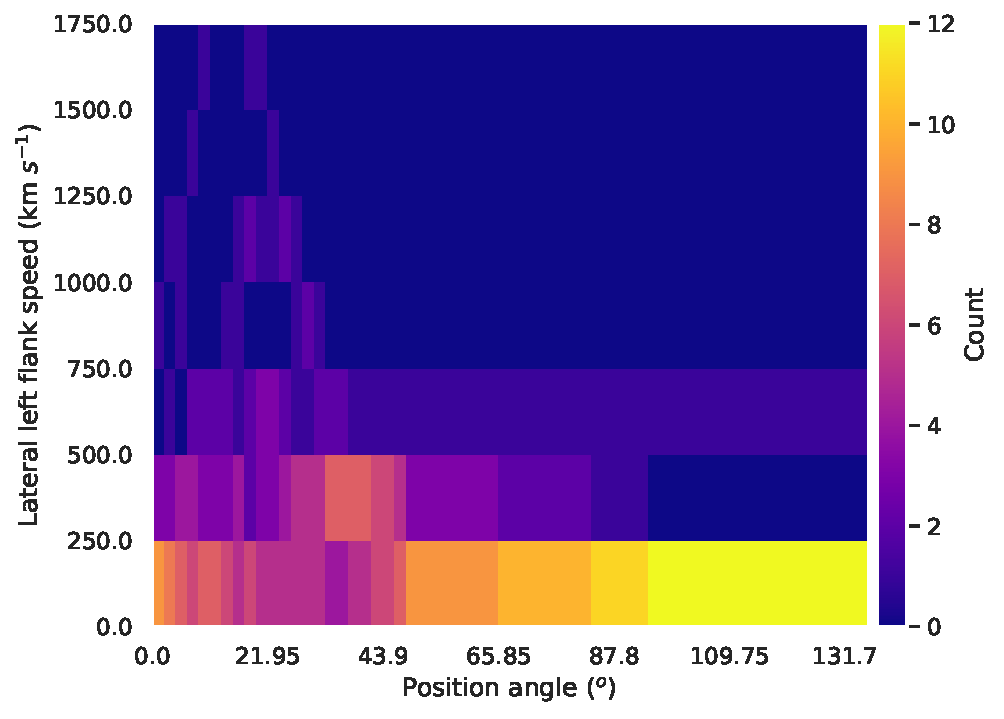
\includegraphics[width=0.32\textwidth,clip=]{chapter2/figs/latleftspd_vs_latleftpos.pdf}
		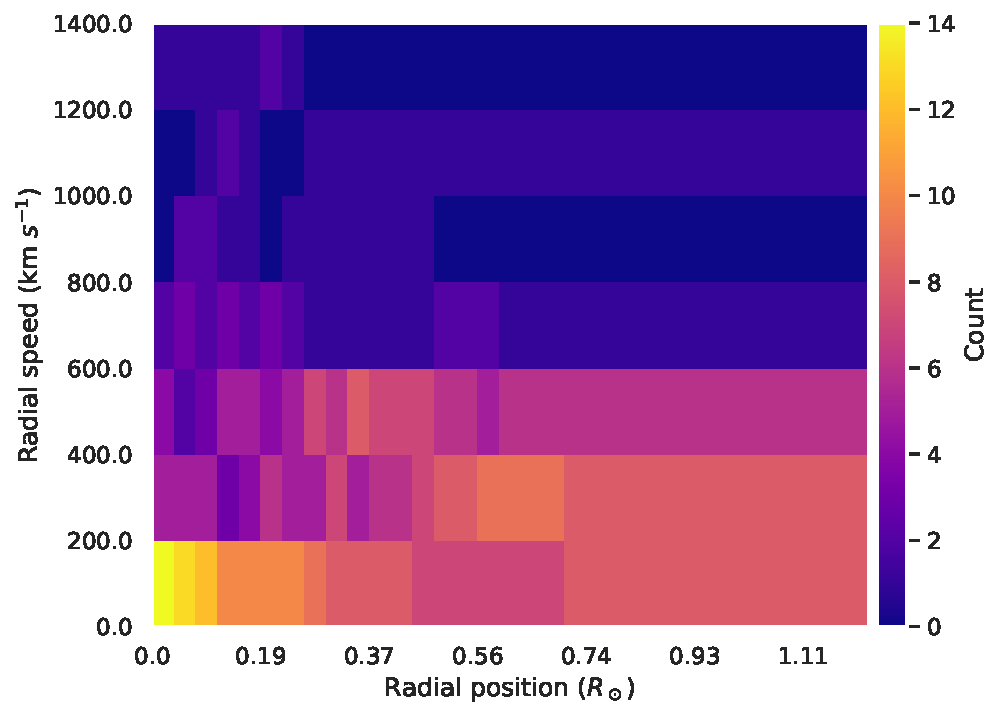
\includegraphics[width=0.32\textwidth,clip=]{chapter2/figs/radspd_vs_radpos.pdf}
		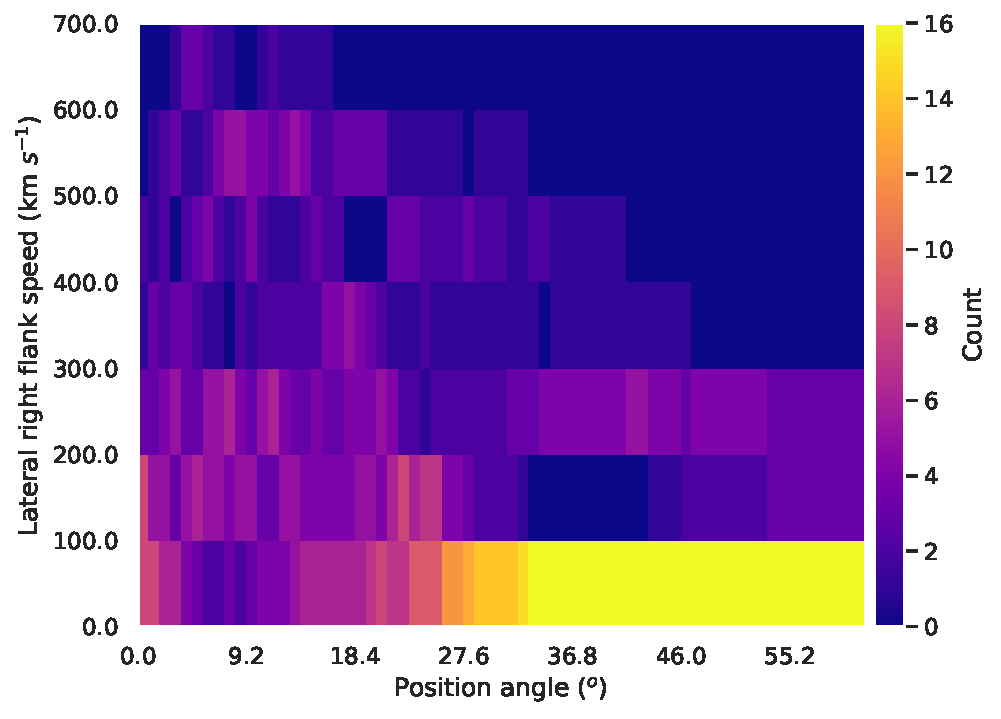
\includegraphics[width=0.32\textwidth,clip=]{chapter2/figs/latrightspd_vs_latrightpos.pdf}
	}
	\centerline{
		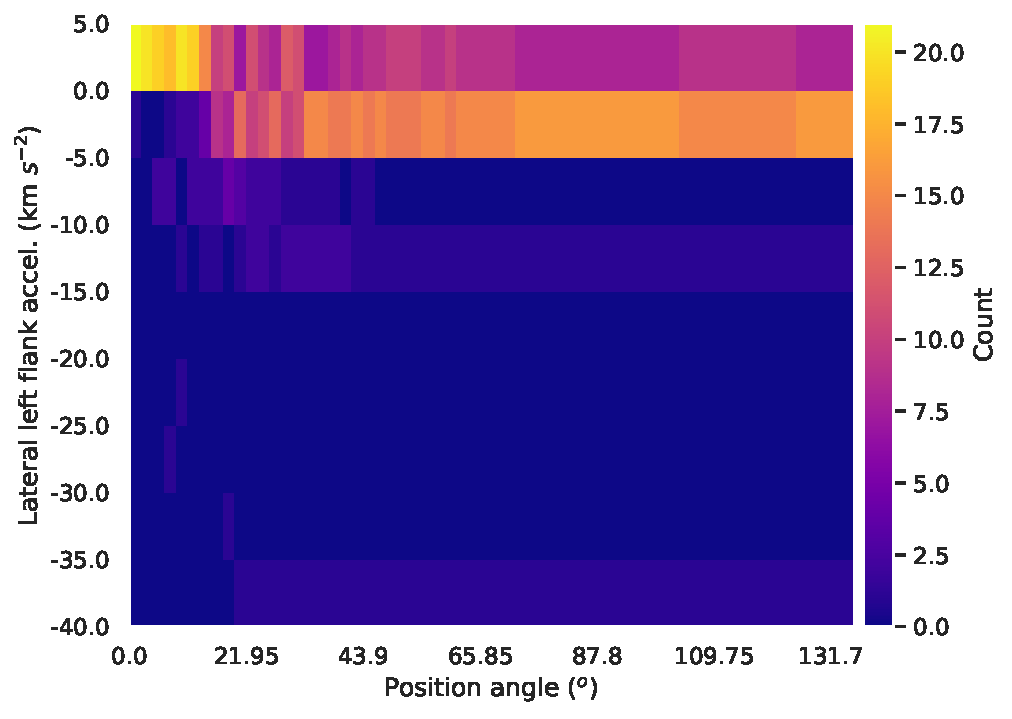
\includegraphics[width=0.32\textwidth,clip=]{chapter2/figs/latleftaccel_vs_latleftpos.pdf}
		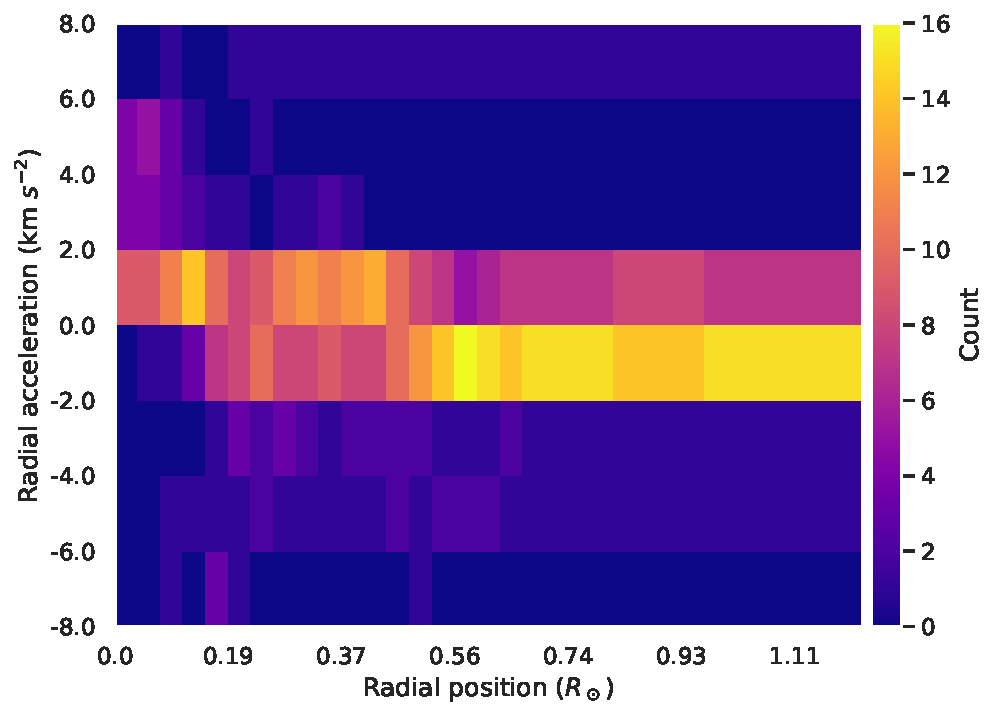
\includegraphics[width=0.32\textwidth,clip=]{chapter2/figs/radaccel_vs_radpos.pdf}
		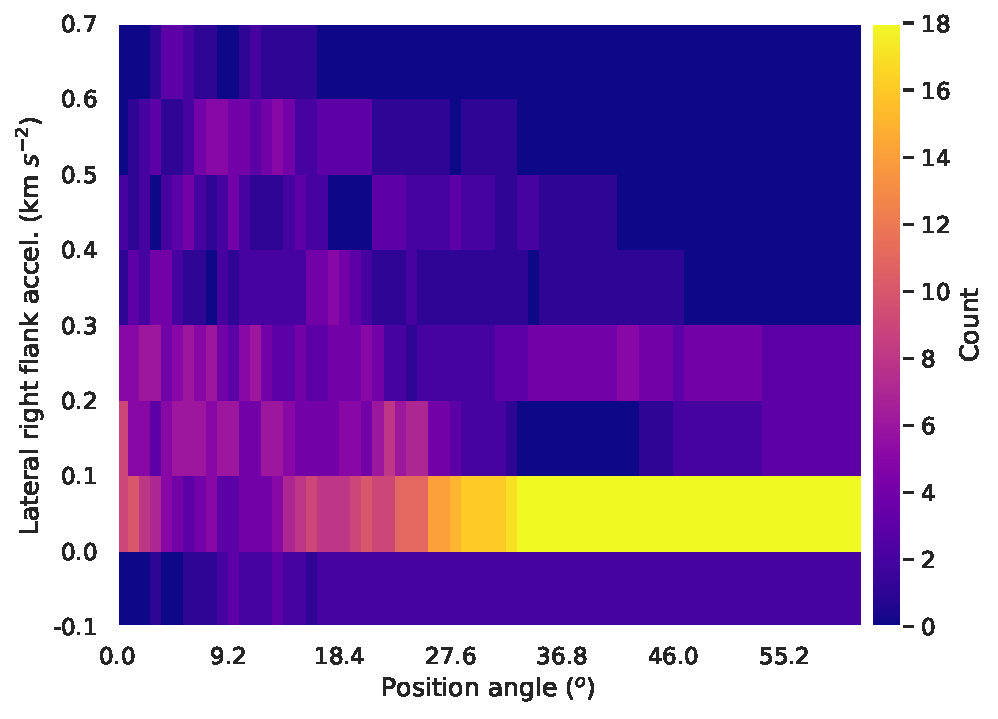
\includegraphics[width=0.32\textwidth,clip=]{chapter2/figs/latrightaccel_vs_latrightpos.pdf}
	}
	\centerline{
		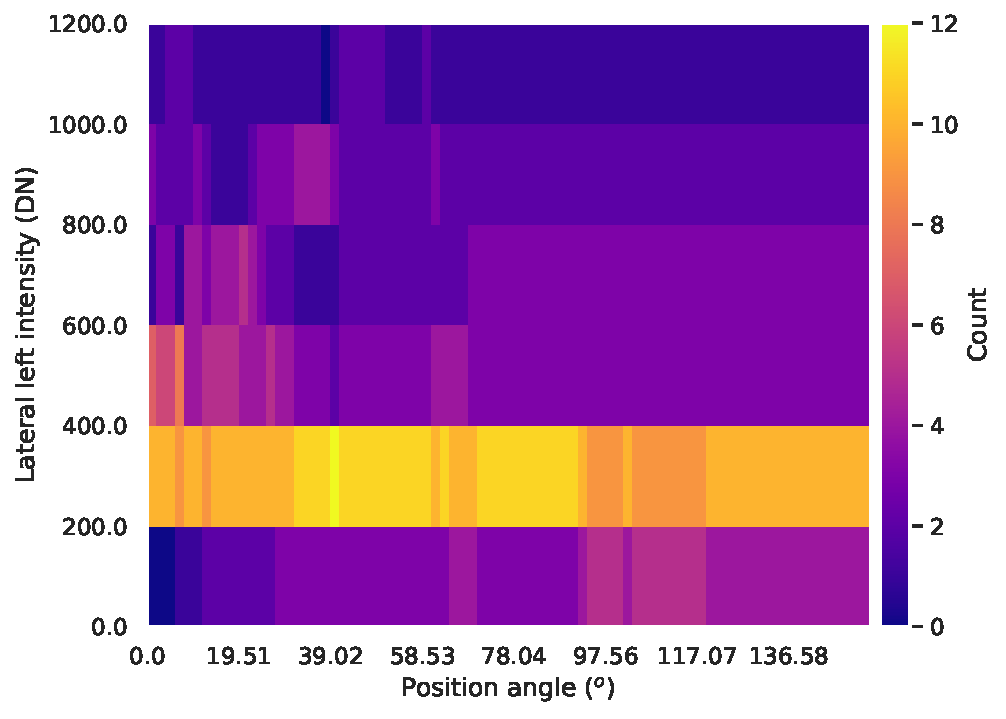
\includegraphics[width=0.32\textwidth,clip=]{chapter2/figs/latleftint_vs_latleftpos.pdf}
		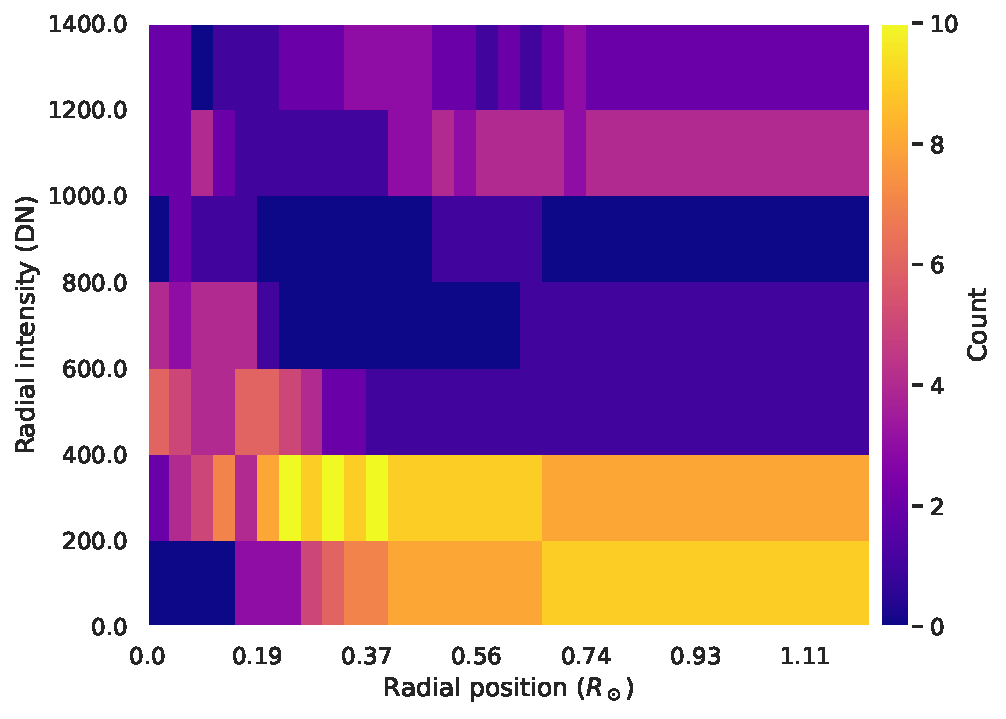
\includegraphics[width=0.32\textwidth,clip=]{chapter2/figs/radint_vs_radpos.pdf}
		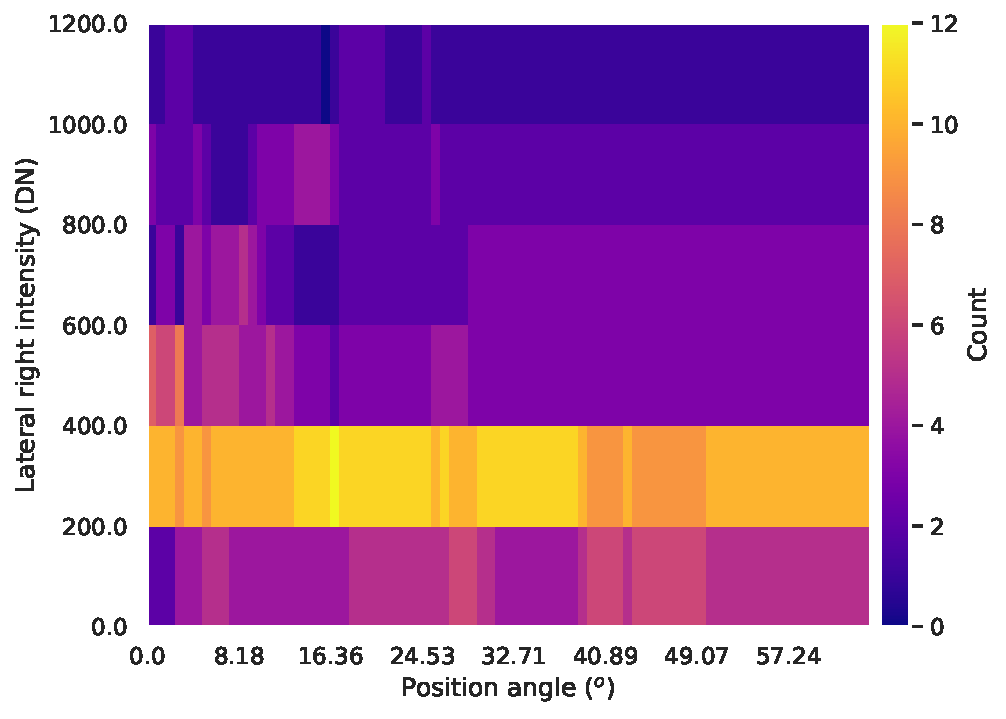
\includegraphics[width=0.32\textwidth,clip=]{chapter2/figs/latrightint_vs_latrightpos.pdf}
	}
	\centerline{
		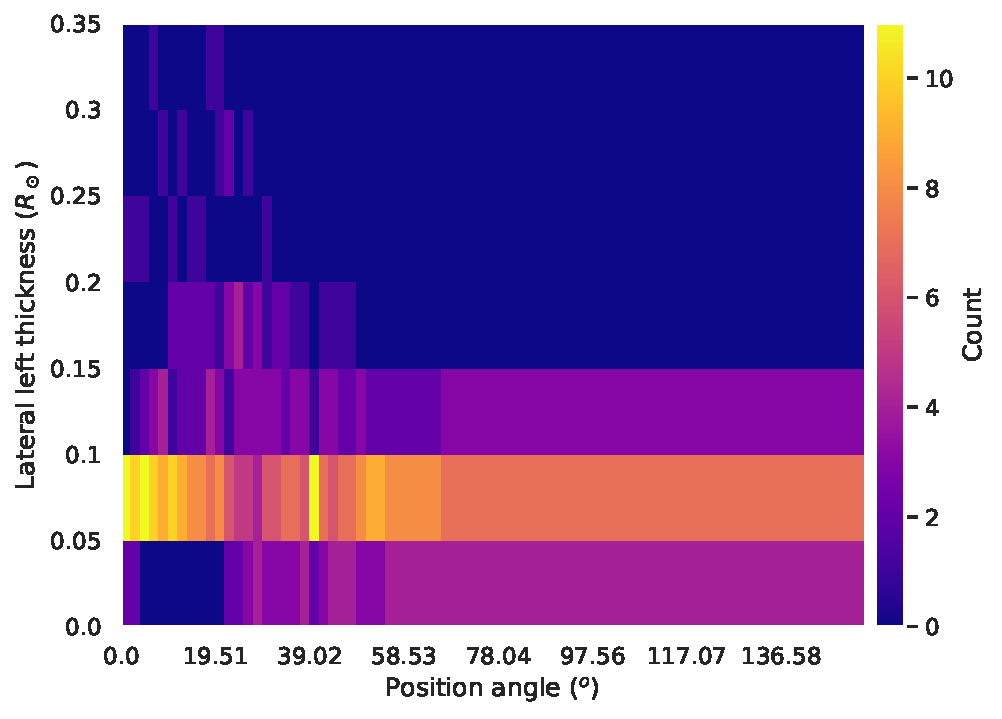
\includegraphics[width=0.32\textwidth,clip=]{chapter2/figs/latleftthick_vs_latleftpos.pdf}
		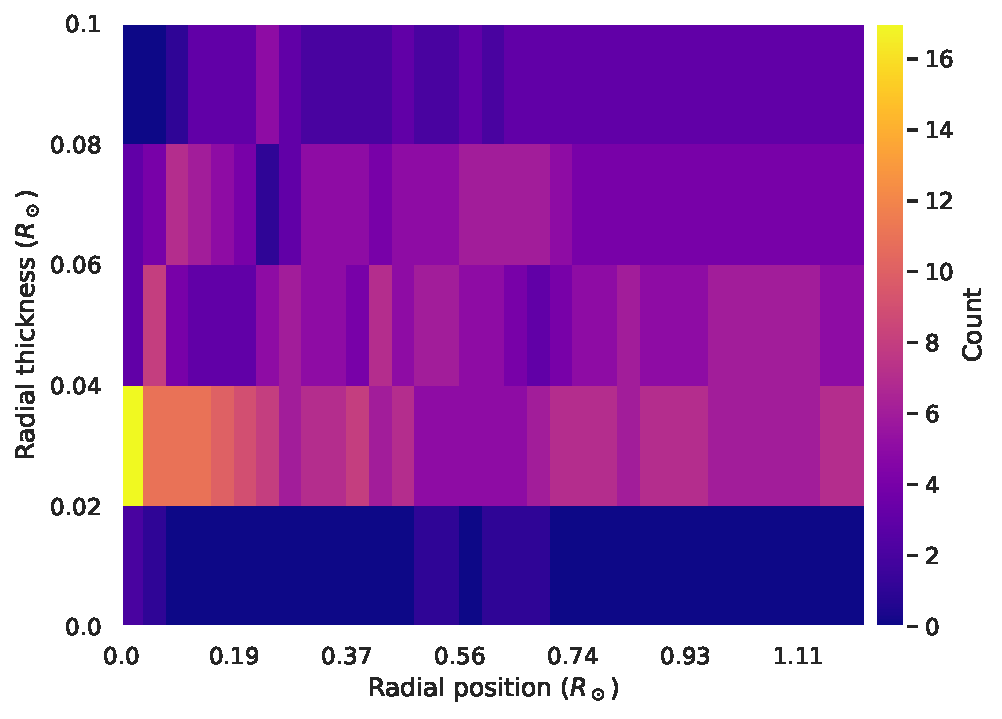
\includegraphics[width=0.32\textwidth,clip=]{chapter2/figs/radthick_vs_radpos.pdf}
		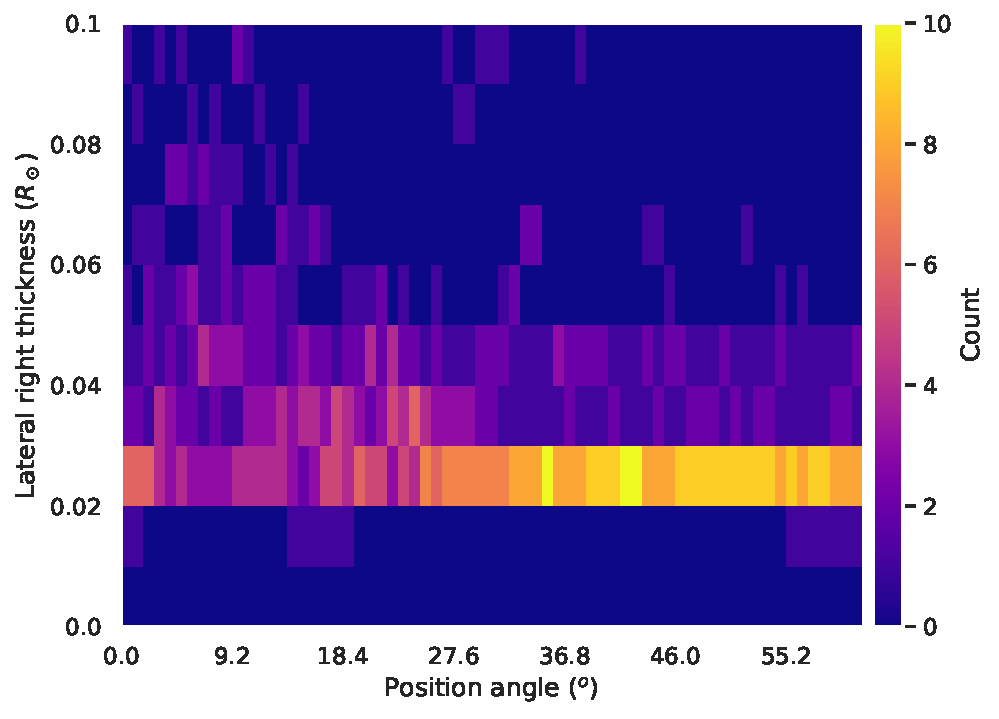
\includegraphics[width=0.32\textwidth,clip=]{chapter2/figs/latrightthick_vs_latrightpos.pdf}
	}
	\caption{Dynamic spectra of the EUV waves kinematics in the AIA FOV. The panels from the top to the bottom are the wave speeds, acceleration, mean intensity, and thickness. The left column is for the lateral left flank, the central column is for the radial direction, and the right column is for the lateral right flank.}
	\label{fig_kinematics_spect_hist}
\end{figure}

Histograms in Figure~\ref{fig_hist_plasma_param_corr} depict correlations between shock-field angle "\textit{THBN}", coronal magnetic field "\textit{BMAG}", plasma density "\textit{DENSITY}" Alfven speed "\textit{VA}", shock speed, and shock density jump "\textit{SHOCKJUMP}".
Moderate positive correlations exist between magnetic field and density, and between magnetic field and Alfven speed, suggesting common underlying physical processes.
A negative correlation between magnetic field and shock density jump implies stronger magnetic fields associate with smaller density jumps across shock surfaces, possibly due to magnetic field pressure resisting plasma compression or faster Alfven waves mitigating density jumps.
Further exploration is warranted to establish definitive connections and parameterize shock density jumps.

\begin{figure}[!htp] % updated!
	\centerline{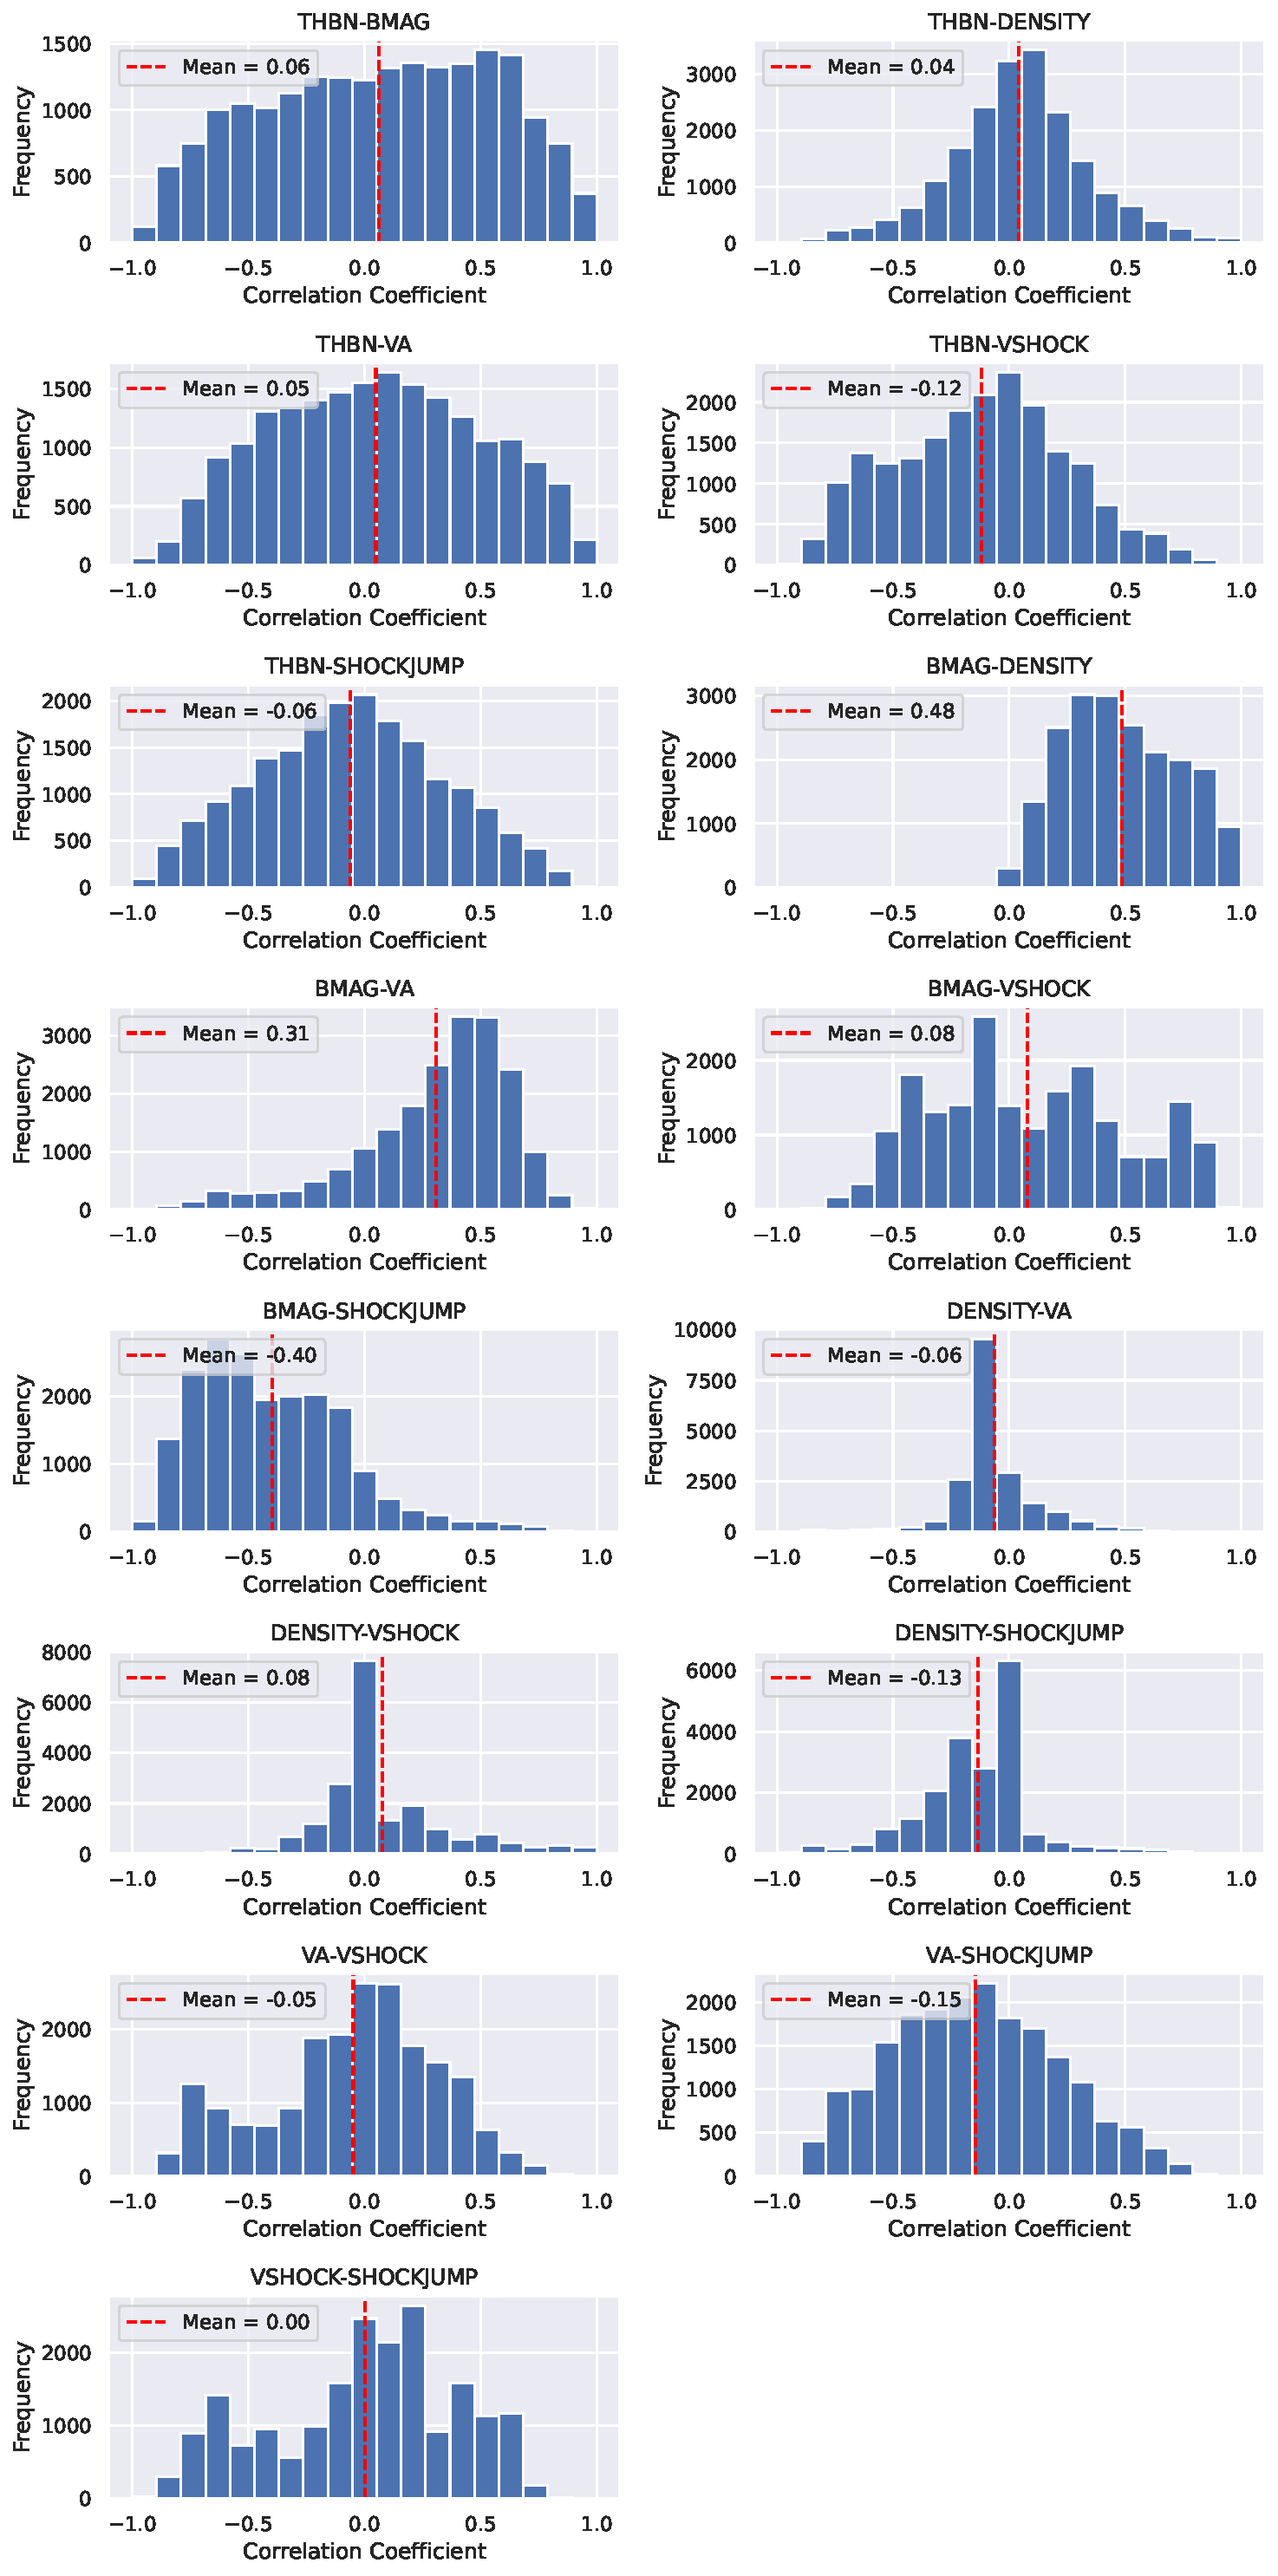
\includegraphics[width=0.7\columnwidth]{chapter2/figs/wp3_d2_Fig16.pdf}}
	\caption{Histograms of along-field-lines model plasma parameters in the solar corona for all the 26 events. The vertical dashed red lines are the mean values.}
	\label{fig_hist_plasma_param_corr}
\end{figure}

\section{Conclusions}
I conducted a study characterizing 26 historical CME-driven CBFs in the low solar corona, observed with the AIA instrument onboard the SDO spacecraft. Utilizing the SPREAdFAST framework, we integrated physics-based and data-driven models to estimate coronal magnetic fields, shock wave dynamics, energetic particle acceleration, and SEP propagation. The analysis relied on AIA base-difference images to generate annulus plots and J-maps for kinematic measurements in radial and lateral directions.

Various time-dependent and distance-dependent kinematic parameters were computed, including shock speed, acceleration, intensity, and thickness. LASCO measurements up to 17$R_{\odot}$ were incorporated to improve SEP spectra characterization. Kinematic measurements facilitated time-dependent 3D geometric models of wavefronts and informed plasma diagnostics through MHD and DEM models.

Shock kinematic measurements were used to fit geometric spheroid surface models for each time step, capturing shock characteristics accurately. Parametrized relationships between plasma parameters were explored to identify connections and interdependencies.

The findings contribute to understanding shock kinematics and plasma parameters. Future investigations will focus on SEP acceleration near the Sun and transport of coronal and interplanetary particles, refining shock and coronal parameter characterization methods for enhanced accuracy and reliability.